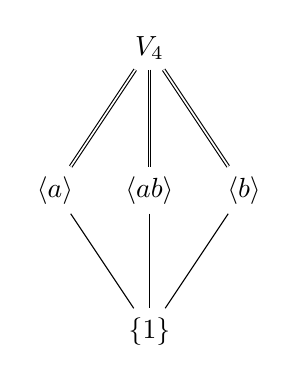
\begin{tikzpicture}[scale=1.2]
  % Nodes
  \node (V4) at (0,3) {$V_4$};

  \node (a) at (-1,1.5) {$\langle a\rangle $};
  \node (ab) at (0,1.5) {$\langle ab \rangle$};
  \node (b) at (1,1.5) {$\langle b \rangle$};

  \node (e) at (0,0) {$\{1\}$};

  % Edges from top
  \draw[double] (V4) -- (a);
  \draw[double] (V4) -- (ab);
  \draw[double] (V4) -- (b);

  % Edges to trivial subgroup
  \draw (a) -- (e);
  \draw (ab) -- (e);
  \draw (b) -- (e);

\end{tikzpicture}
